% This is "sig-alternate.tex" V2.1 April 2013
% This file should be compiled with V2.5 of "sig-alternate.cls" May 2012
%
% This example file demonstrates the use of the 'sig-alternate.cls'
% V2.5 LaTeX2e document class file. It is for those submitting
% articles to ACM Conference Proceedings WHO DO NOT WISH TO
% STRICTLY ADHERE TO THE SIGS (PUBS-BOARD-ENDORSED) STYLE.
% The 'sig-alternate.cls' file will produce a similar-looking,
% albeit, 'tighter' paper resulting in, invariably, fewer pages.
%
% ----------------------------------------------------------------------------------------------------------------
% This .tex file (and associated .cls V2.5) produces:
%       1) The Permission Statement
%       2) The Conference (location) Info information
%       3) The Copyright Line with ACM data
%       4) NO page numbers
%
% as against the acm_proc_article-sp.cls file which
% DOES NOT produce 1) thru' 3) above.
%
% Using 'sig-alternate.cls' you have control, however, from within
% the source .tex file, over both the CopyrightYear
% (defaulted to 200X) and the ACM Copyright Data
% (defaulted to X-XXXXX-XX-X/XX/XX).
% e.g.
% \CopyrightYear{2007} will cause 2007 to appear in the copyright line.
% \crdata{0-12345-67-8/90/12} will cause 0-12345-67-8/90/12 to appear in the copyright line.
%
% ---------------------------------------------------------------------------------------------------------------
% This .tex source is an example which *does* use
% the .bib file (from which the .bbl file % is produced).
% REMEMBER HOWEVER: After having produced the .bbl file,
% and prior to final submission, you *NEED* to 'insert'
% your .bbl file into your source .tex file so as to provide
% ONE 'self-contained' source file.
%
% ================= IF YOU HAVE QUESTIONS =======================
% Questions regarding the SIGS styles, SIGS policies and
% procedures, Conferences etc. should be sent to
% Adrienne Griscti (griscti@acm.org)
%
% Technical questions _only_ to
% Gerald Murray (murray@hq.acm.org)
% ===============================================================
%
% For tracking purposes - this is V2.0 - May 2012

\documentclass{sig-alternate-05-2015}


\begin{document}

% Copyright
\setcopyright{acmcopyright}
%\setcopyright{acmlicensed}
%\setcopyright{rightsretained}
%\setcopyright{usgov}
%\setcopyright{usgovmixed}
%\setcopyright{cagov}
%\setcopyright{cagovmixed}

%
% --- Author Metadata here ---
%\CopyrightYear{2007} % Allows default copyright year (20XX) to be over-ridden - IF NEED BE.
%\crdata{0-12345-67-8/90/01}  % Allows default copyright data (0-89791-88-6/97/05) to be over-ridden - IF NEED BE.
% --- End of Author Metadata ---

\title{Twitter Bot Behavior: How Twitter Bots Interact With People}
\subtitle{}
%
% You need the command \numberofauthors to handle the 'placement
% and alignment' of the authors beneath the title.
%
% For aesthetic reasons, we recommend 'three authors at a time'
% i.e. three 'name/affiliation blocks' be placed beneath the title.
%
% NOTE: You are NOT restricted in how many 'rows' of
% "name/affiliations" may appear. We just ask that you restrict
% the number of 'columns' to three.
%
% Because of the available 'opening page real-estate'
% we ask you to refrain from putting more than six authors
% (two rows with three columns) beneath the article title.
% More than six makes the first-page appear very cluttered indeed.
%
% Use the \alignauthor commands to handle the names
% and affiliations for an 'aesthetic maximum' of six authors.
% Add names, affiliations, addresses for
% the seventh etc. author(s) as the argument for the
% \additionalauthors command.
% These 'additional authors' will be output/set for you
% without further effort on your part as the last section in
% the body of your article BEFORE References or any Appendices.

\numberofauthors{2} %  in this sample file, there are a *total*
% of EIGHT authors. SIX appear on the 'first-page' (for formatting
% reasons) and the remaining two appear in the \additionalauthors section.
%
\author{
% You can go ahead and credit any number of authors here,
% e.g. one 'row of three' or two rows (consisting of one row of three
% and a second row of one, two or three).
%
% The command \alignauthor (no curly braces needed) should
% precede each author name, affiliation/snail-mail address and
% e-mail address. Additionally, tag each line of
% affiliation/address with \affaddr, and tag the
% e-mail address with \email.
%
% 1st. author
\alignauthor
Alic Szecsei\\
       \affaddr{University of Iowa}\\
       \email{alic-szecsei@uiowa.edu}
% 2nd. author
\alignauthor
Willem DeJong\\
       \affaddr{University of Iowa}\\
       \email{willem-dejong@uiowa.edu}
}

\maketitle
\begin{abstract}
% ABSTRACT (up to 200 words)
Twitter bots are often cited as affecting the political process by manipulating the trending topics data; similar behavior is also cited on other social platforms, such as Facebook. We present our use of unsupervised machine learning, combined with Indiana University's \emph{BotOrNot} service, to classify Twitter users as bots based on statistical analysis of their accounts, and then examine the ways in which they interact with other users. Determining how these bots interact with human users can help to focus bot-detection algorithms to target those bots that interact with human users in malicious ways.
\end{abstract}

% We no longer use \terms command
%\terms{Theory}

\section{Introduction}
% 1. INTRODUCTION (1 page)

\subsection{Background \& Motivation}
% 1.1 Background & Motivation (1-2 paragraphs)
\emph{Social bots}, also known as \emph{sybil accounts}, are programs that automate interaction on social platforms. While some may simply be humorous or helpful accounts that don't attempt to hide their status as bots, others have more manipulative goals; they may flood a social network with spam, or attempt to more subtly influence the thoughts and behavior of the humans it interacts with. While social networks are extremely effective at causing social change and improving the quality of life of their users, they are also at risk of automated manipulation by bots.

Aral and Walker (2011) showed that social networks are highly effective at manipulating the public\cite{Aral:Contagion}, and the automation of such behavior only increases this efficiency. In addition, Ratkiewicz (2011) showed that political bots actively manipulated the 2010 U.S. midterm elections\cite{Ratkiewicz:PoliticalAbuse}.

\subsection{Problem Statement}
% 1.2 Problem Statement (1 paragraph)
While there have been multiple approaches to bot detection\cite{Stringhini:DetectSpam}\cite{Xiao:ClusterFakeAccounts}\cite{Chu:DetectAutomation}, these have been restrained to simple detection. Very few have attempted to examine the ways that these fake accounts interact with real users. Our goal is to find a number of bot accounts and determine how they use social media to affect their target users. Determining which bots are attempting to manipulate social networks and which are providing services to human users is an import aspect of bot detection, and one we believe can be improved by examining how malicious bots interact with human users.

\subsection{Proposed Approach}
% 1.3 Proposed Approach (1 paragraph)
In this paper, we use data from a bot-detection service run by Indiana University to determine whether or not users are bots. We then pull their latest tweets, as well as user data, and use the collected data in an unsupervised machine learning algorithm to cluster the users into 50 groups. We then take the data for each cluster and analyze common behavioral patterns.

\subsection{Key Results}
% 1.4 Key Results (1-2 paragraph)
We found a general inverse trend between the \emph{BotOrNot} score for a cluster and the number of retweets made by the cluster. In addition, a similar inverse trend exists for the number of links tweeted by users, and the number of mentions made by users.

Lorem ipsum lorem ipsum lorem ipsum lorem ipsum lorem ipsum lorem ipsum lorem ipsum lorem ipsum lorem ipsum lorem ipsum lorem ipsum lorem ipsum lorem ipsum lorem ipsum lorem ipsum lorem ipsum lorem ipsum lorem ipsum lorem ipsum lorem ipsum lorem ipsum lorem ipsum lorem ipsum lorem ipsum lorem ipsum lorem ipsum lorem ipsum lorem ipsum lorem ipsum lorem ipsum lorem ipsum lorem ipsum lorem ipsum lorem ipsum.

\section{Related Work}
% RELATED WORK (1/2 page)
Davis (2016)\cite{Davis:BotOrNot} and Dickerson (2014)\cite{Dickerson:Sentiment}. [TODO: Talk about cited papers, what their results were, how those results were relevant to our data] Lorem ipsum lorem ipsum lorem ipsum lorem ipsum lorem ipsum lorem ipsum lorem ipsum lorem ipsum lorem ipsum lorem ipsum lorem ipsum lorem ipsum lorem ipsum lorem ipsum lorem ipsum lorem ipsum lorem ipsum lorem ipsum lorem ipsum lorem ipsum lorem ipsum lorem ipsum lorem ipsum lorem ipsum lorem ipsum lorem ipsum lorem ipsum lorem ipsum lorem ipsum lorem ipsum lorem ipsum lorem ipsum lorem ipsum lorem ipsum.

Lorem ipsum lorem ipsum lorem ipsum lorem ipsum lorem ipsum lorem ipsum lorem ipsum lorem ipsum lorem ipsum lorem ipsum lorem ipsum lorem ipsum lorem ipsum lorem ipsum lorem ipsum lorem ipsum lorem ipsum lorem ipsum lorem ipsum lorem ipsum lorem ipsum lorem ipsum lorem ipsum lorem ipsum lorem ipsum lorem ipsum lorem ipsum lorem ipsum lorem ipsum lorem ipsum lorem ipsum lorem ipsum lorem ipsum lorem ipsum

Lorem ipsum lorem ipsum lorem ipsum lorem ipsum lorem ipsum lorem ipsum lorem ipsum lorem ipsum lorem ipsum lorem ipsum lorem ipsum lorem ipsum lorem ipsum lorem ipsum lorem ipsum lorem ipsum lorem ipsum lorem ipsum lorem ipsum lorem ipsum lorem ipsum lorem ipsum lorem ipsum lorem ipsum lorem ipsum lorem ipsum lorem ipsum lorem ipsum lorem ipsum lorem ipsum lorem ipsum lorem ipsum lorem ipsum lorem ipsum.

Lorem ipsum lorem ipsum lorem ipsum lorem ipsum lorem ipsum lorem ipsum lorem ipsum lorem ipsum lorem ipsum lorem ipsum lorem ipsum lorem ipsum lorem ipsum lorem ipsum lorem ipsum lorem ipsum lorem ipsum lorem ipsum lorem ipsum lorem ipsum lorem ipsum lorem ipsum lorem ipsum lorem ipsum lorem ipsum lorem ipsum lorem ipsum lorem ipsum lorem ipsum lorem ipsum lorem ipsum lorem ipsum lorem ipsum lorem ipsum.

Lorem ipsum lorem ipsum lorem ipsum lorem ipsum lorem ipsum lorem ipsum lorem ipsum lorem ipsum lorem ipsum lorem ipsum lorem ipsum lorem ipsum lorem ipsum lorem ipsum lorem ipsum lorem ipsum lorem ipsum lorem ipsum lorem ipsum lorem ipsum lorem ipsum lorem ipsum lorem ipsum lorem ipsum lorem ipsum lorem ipsum lorem ipsum lorem ipsum lorem ipsum lorem ipsum lorem ipsum lorem ipsum lorem ipsum lorem ipsum.

\section{Proposed Approach}
% PROPOSED APPROACH (1 page)
Many examinations of bot behavior on Twitter uses ground truths created by verified accounts. However, the social behavior of verified Twitter accounts is wildly different from that of the general public. Verified users often have a celebrity status, and so are less likely to retweet other users, and usually will not have a small number of followers.

In addition, verified Twitter accounts occasionally belong to people who exhibit bot-like behavior, advertising their services without much variety between tweets, and consistently linking to their personal websites. While these users may be verified, they are not guaranteed to be run by real people, and are often linked to other services to simply tweet links.

Instead, we chose to start with Twitter accounts we knew or who followed our personal accounts, and then attempt to provide a more detailed classification system to account for these "`verified bots."'

To retrieve a list of human and bot Twitter accounts, we compiled an initial list of 113 users with an approximately even split between humans and bots. We then retrieved data for their followers, and their followers' followers, leaving us with 9,025 Twitter users, which we then classified.

\subsection{Clustering}

\emph{BotOrNot} analyzes a large amount of data retrieved from each user, including sentiment analysis and a temporal analysis to determine when users are likely to tweet. Using machine learning classifiers, it assigns a score to a user, with higher scores indicating a larger amount of bot-like behavior.

Testing \emph{BotOrNot} lead us to discover a number of inconsistencies with the overall score. A Twitter bot owned by one of the authors was given a lower score than the personal account that the bot was attempting to imitate. Organizational accounts were often given a high \emph{BotOrNot} score, which the official website discloses. One account was owned by the son of another user, who had only made 3 tweets and had a \emph{BotOrNot} score of over 90%.

After discovering these issues, we determined that more information was required for automated analysis of Twitter accounts. Using unsupervised machine learning to cluster accounts let us successfully organize a large number of accounts into separate categories, which we manually classified and verified. As described by Bessi and Ferrera\cite{Bessi:PresElect}, we retrieved the most important descriptors of bots: whether they're using the default appearance, their retweet-to-tweet ratio, and others, in addition to the \emph{BotOrNot} score and category scores. However, our best results were found when simply clustering based on the \emph{BotOrNot} category scores.

To classify each cluster, we set up a basic Python script using Selenium that displayed a sample set of Twitter feeds, and allowed a user to submit a category for the user. Based on the categories reported for the cluster, we could determine what type of Twitter account a user was likely to be. We then manually categorized approximately [TODO: Number] 750 of these accounts, split evenly among each cluster.

\subsection{Tweet Analysis}

We determined how bots could engage with human users on the Twitter platform, determining that these vectors consisted of:
\begin{itemize}
	\item Mentioning a user in a tweet
	\item Retweeting a user
	\item Using a popular hashtag or phrase
	\item Following a user
	\item Favoriting another user's tweet
\end{itemize}
We collected data about how many accounts each account was following, how many accounts followed them, and how many tweets each account had favorited. This user data let us analyze how many accounts each cluster was following, and helped manually classify certain users as bots.

In addition to retrieving this user data, the latest tweets made by each account, with a total of over 1 million tweets. We could then determine whether the tweet had been retweeted from another user, contained links, mentioned other users, and which hashtags were used.

Using these social behaviors, we were able to determine how each cluster and category of user tended to interact with other users. Focusing bot detection on these interactions could result in improved efficiency for spam removal services or other bot-related studies.

\section{Results \& Discussion}
% RESULTS & DISCUSSIONS (3 pages including tables and figures)

Examining the correctness of \emph{BotOrNot} scoring was the first part of analysis we performed. Manually determining whether a number of accounts were bots, humans, or indeterminate, we found that the majority of accounts with a \emph{BotOrNot} score over 50\% we were unable to determine if the account was automated, or the account was clearly a bot. Likewise, the majority of accounts with a score less than 50\% were clearly human users, as seen in Figures \ref{fig:scorescat} and \ref{fig:barvsaccnt}.

\begin{figure}
	\caption{Manual identification of accounts}
	\centering
		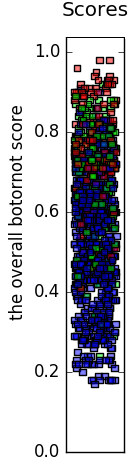
\includegraphics[width=0.4\textwidth]{imgs/scorenbotcolor}
	\label{fig:scorescat}
	
\end{figure}

\begin{figure}
	\caption{Manual identification of accounts}
	\centering
		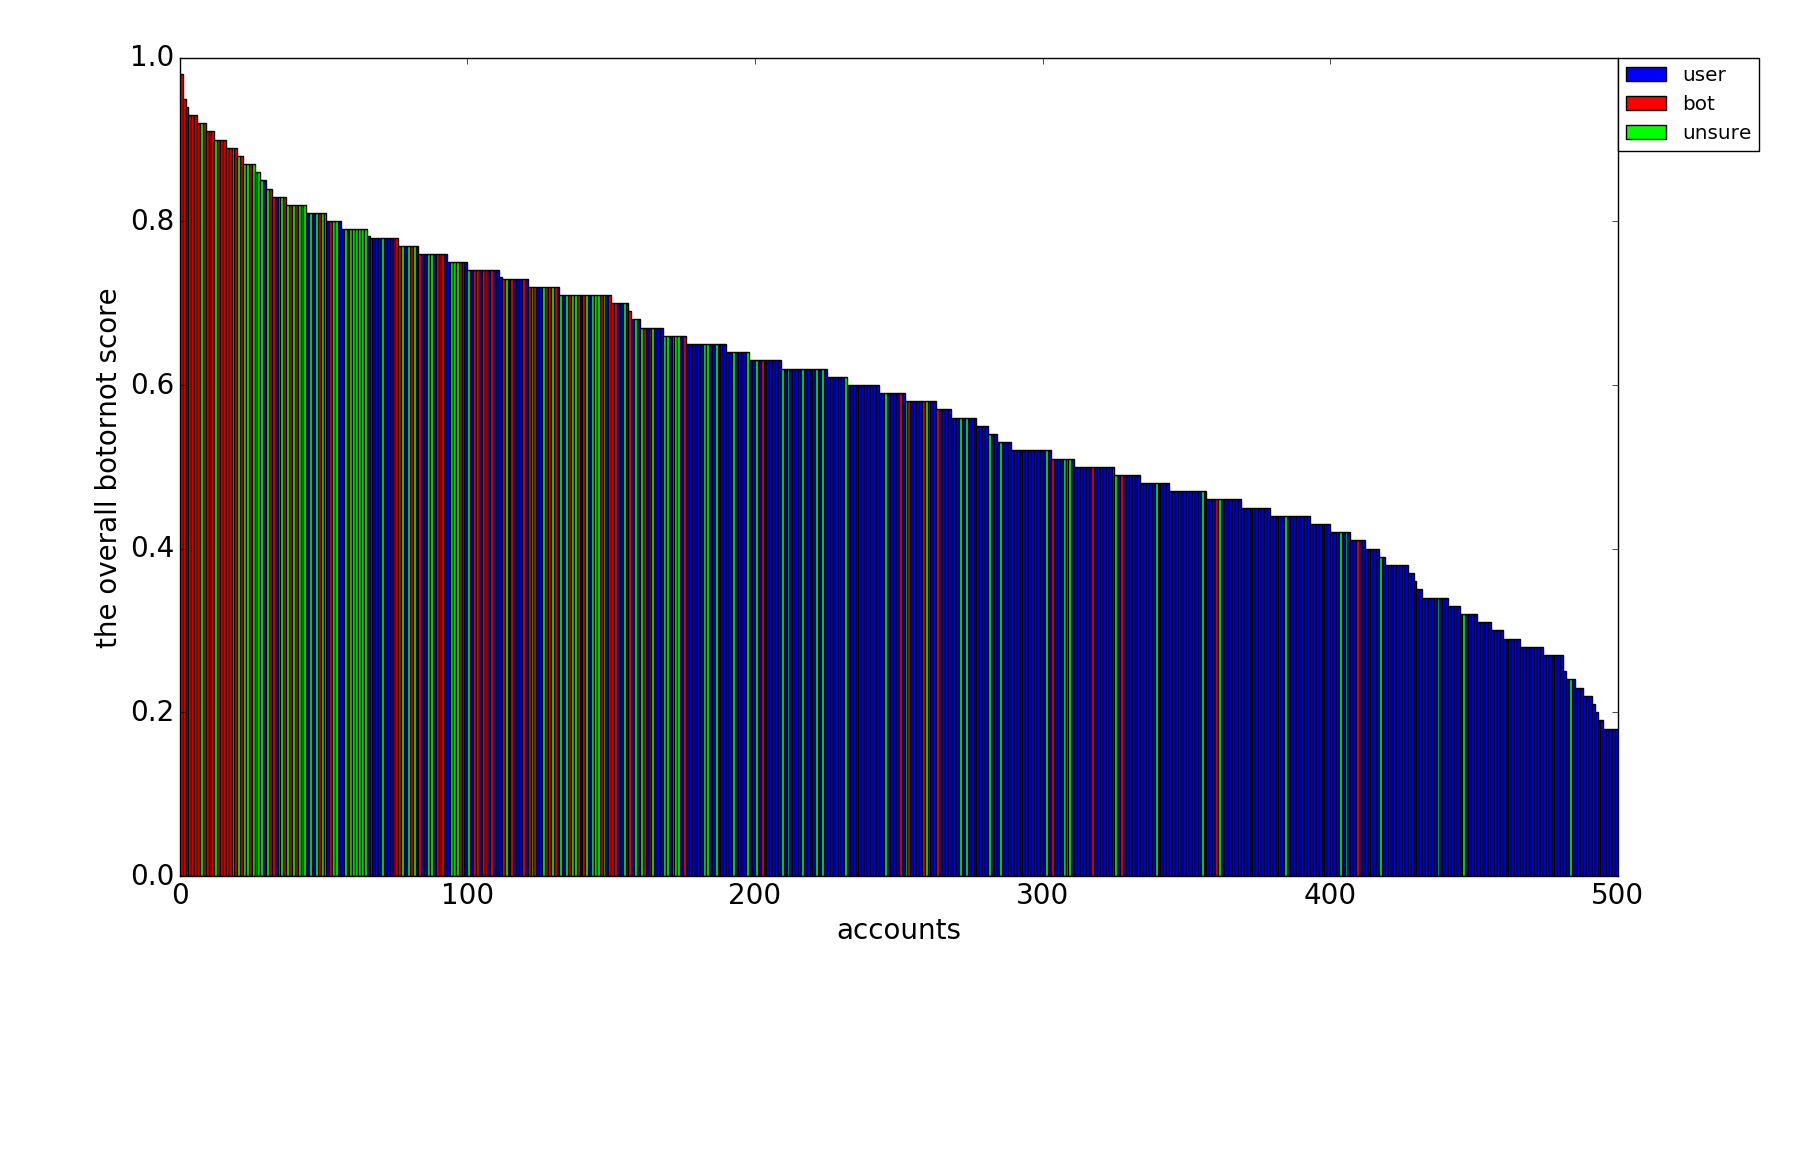
\includegraphics[width=0.6\textwidth]{imgs/barvsaccnt}
	\label{fig:barvsaccnt}
\end{figure}

We next examined how \emph{BotOrNot}'s category subscores aligned with its overall account score.

\begin{figure}
	\caption{\emph{BotOrNot} Scores vs Category Subscores}
	\centering
		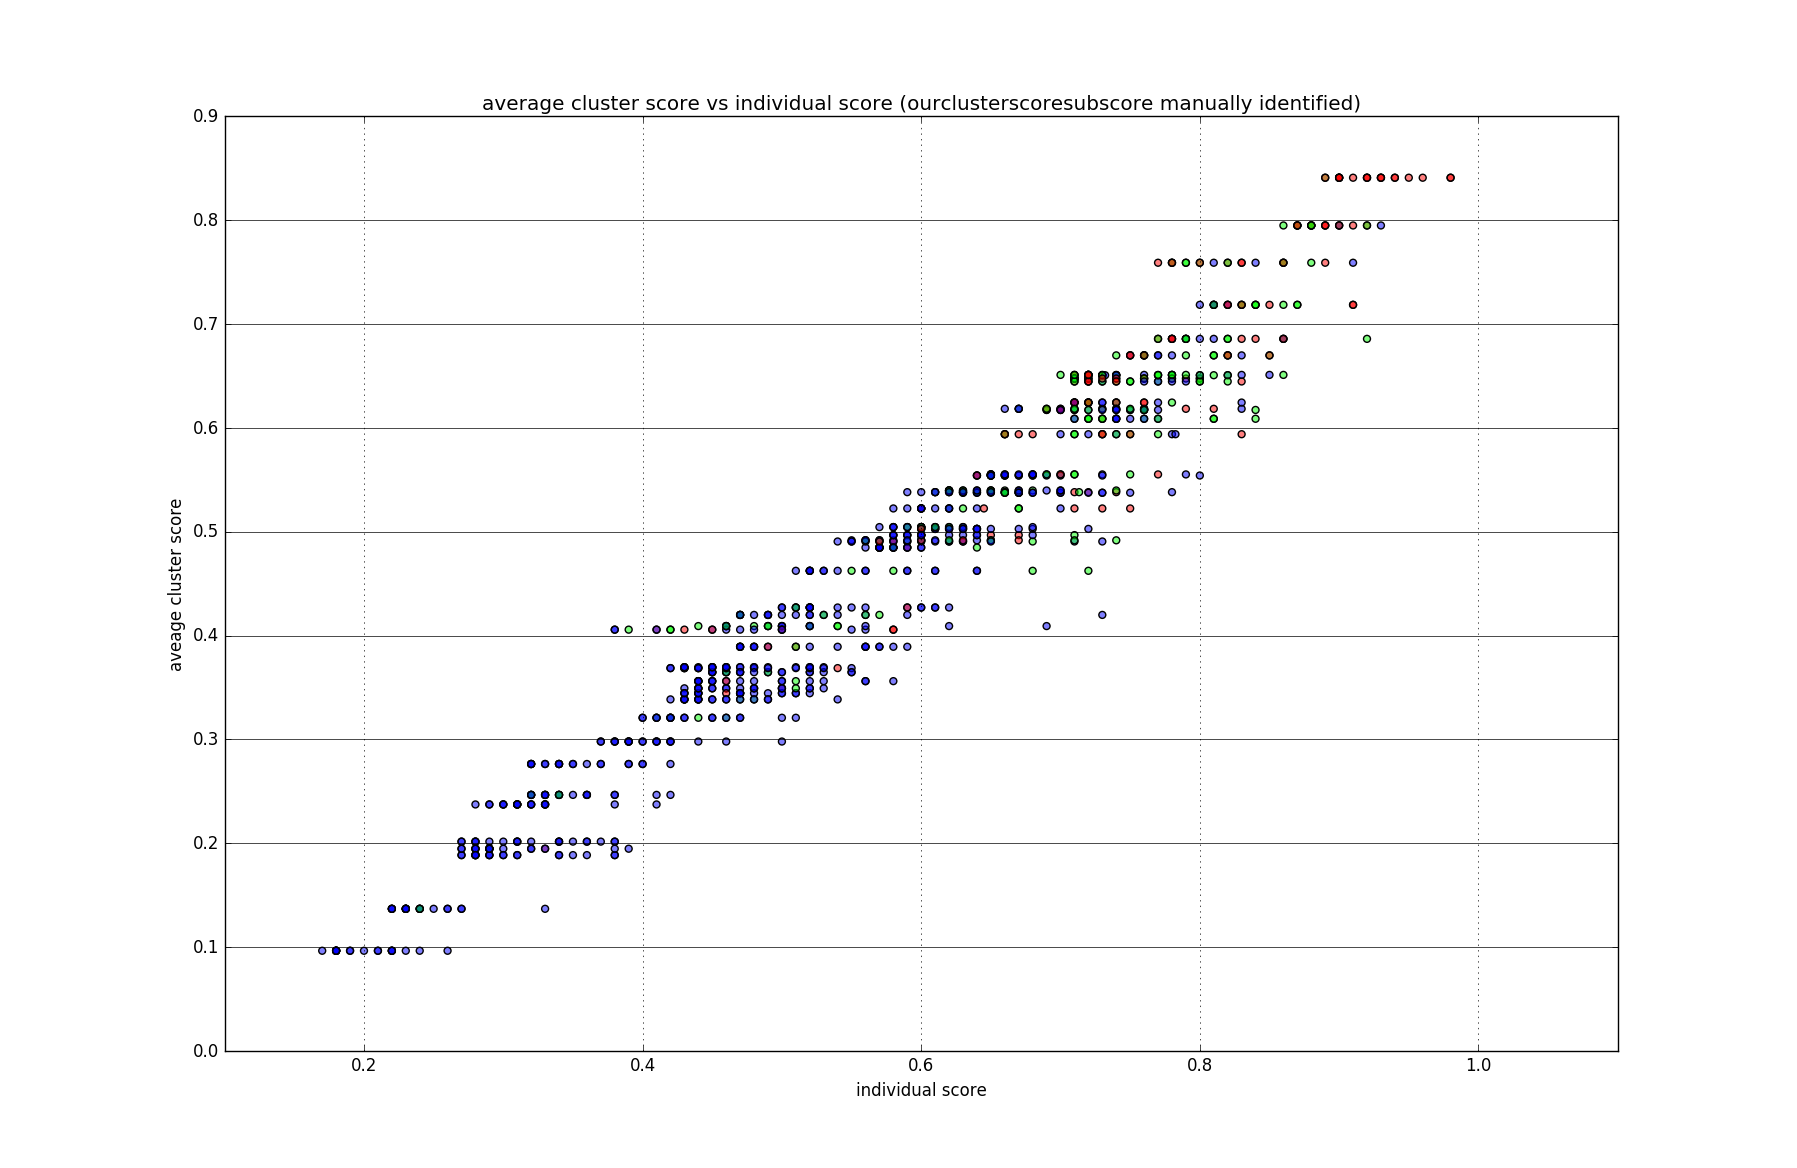
\includegraphics[width=0.6\textwidth]{imgs/ourscorevssubscore}
	\label{fig:scoresubscore}
\end{figure}


\section{Conclusion}
% CONCLUSION (~1/4 pages)
Our study focused on analyzing interaction between human and bot Twitter users. We used \emph{BotOrNot}, combined with unsupervised machine learning, to cluster users and determine how bots gain visibility with their target audience. We determined that bots are unlikely to engage with human users beyond simply following them.

\subsection{Further Work}
Although we were able to manually identify advertising links, when we retrieved data on individual Tweets we did not expand Twitter's shortened URL format. This made media, such as photos, appear identical to other links, since Twitter represents media as URLs. In addition, the sample size for manual classification was small by necessity; setting up a web service such as Mechanical Turk to crowdsource this account classification would improve analysis and clustering.

%
% The following two commands are all you need in the
% initial runs of your .tex file to
% produce the bibliography for the citations in your paper.
\bibliographystyle{abbrv}
\bibliography{sigproc}  % sigproc.bib is the name of the Bibliography in this case
% You must have a proper ".bib" file
%  and remember to run:
% latex bibtex latex latex
% to resolve all references
%
% ACM needs 'a single self-contained file'!
%
%APPENDICES are optional
%\balancecolumns
% \appendix

\appendix
\section{Contributions}
Alic Szecsei provided data retrieval methods for Twitter accounts, programmed the unsupervised machine learning, and wrote the data analysis.

Willem DeJong programmed BotOrNot score retrieval, retrieved data for Twitter accounts to store in SQL databases, and created many of the graphs and charts.

%\balancecolumns % GM June 2007
% That's all folks!
\end{document}
